\documentclass[main.tex]{subfiles}
\begin{document}

% \section*{Fri Oct 11 2019}
\marginpar{Friday \\ 2019-10-11, \\ compiled \\ \today}

% On Oct 31 Marco Peloso will not give his lecture, so Sabino will do both lectures.

% Recalling last lecture: 
% we consider a universe with constant density \(\rho\)\dots

We can also recover the third Friedmann equation 
\begin{equation}
\dot{\rho} = -3 \frac{\dot{a}}{a} \qty(\rho + \frac{P}{c^2}) \approx -3 \frac{\dot{a}}{a} \rho 
\,,
\end{equation}
%
where the approximation as before is the Newtonian one, \(P \ll \rho c^2\). In this case, however, we will be able to also recover the nonrelativistic pressure term if we account for conservation of energy and not just mass.
% without the last term, which yet again will come from the relativistic consideration.

When deriving these equations relativistically the third one comes from the conservation of the temporal component of the stress-energy tensor (\(\nabla_{\mu } T^{\mu 0} = 0\)), i.e. the ``conservation of energy'',\footnote{This is actually \emph{not} a conservation law as stated, it is not covariant: in order for it to be we would need to project it along a temporal Killing vector, which does not exist in cosmology. However, if we did have a temporal Killing vector \(\xi_{\mu }\) the projection \(\xi_{\nu } \nabla_{\mu } T^{\mu \nu } =0\) would indeed be the conservation of energy.

Indeed, it is more correct to say that this equation is not a conservation law at all, but is instead just an expression of the geometric Bianchi identities \(\nabla_{\mu } G^{\mu \nu }=0\), which are written in terms of the Einstein tensor \(G_{\mu \nu } = R_{\mu \nu } - \frac{1}{2} R g_{\mu \nu }\); if the Einstein equations hold then \(G_{\mu \nu } \) is proportional to \(T_{\mu \nu }\), therefore the two statements are equivalent.}
so to find it in our Newtonian calculation we will need to consider the nonrelativistic equivalent of that equation, which is the first law of thermodynamics.

We will consider \emph{ideal fluids}.
The first law, assuming adiabaticity --- which must be present, since net heat transfer in the universe would violate isotropy ---  states:
\begin{equation}
  \dd{E} + P\dd{V} = 0\,.
\end{equation}

We can write the total energy as the product of the energy density times the volume: \(E = \frac{4 \pi }{3} \rho c^2 a^{3}\), since the volume is \(V = \frac{4 \pi }{3} a^3\).

So, the first law reads: 
%
\begin{align}
0&=\frac{4\pi }{3}\qty[\dd{\qty(\rho c^2 a^3)} + P \dd{(a^3)}]   \\
&= c^2 \rho \dd{(a^3)} + c^2 a^3 \dd{\rho } + P \dd{(a^3)}   \marginnote{Divided through by \(4 \pi / 3\)}\\
&= 3 \qty(\rho + \frac{P}{c^2}) \frac{\dd{a}}{a} + \dd{\rho } \marginnote{Divided through by \(c^2a^3\), collected terms.}
\,,
\end{align}
%
which is the third Friedmann equation, \eqref{eq:friedmann-3}: the only manipulation left to do is to apply the differentials, which are covectors, to the temporal vector \(\dv*{}{t}\) in order to turn them into time derivatives.

Why were we able to recover the relativistic term this time? The completely non-relativistic approach to this would be to write \(M = \frac{4\pi }{3} \rho a^3 \), and to write down the equation for the conservation of mass alone. 
Indeed, this would yield the Friedmann equation without the \(P\) term.

\todo[inline]{Footnote number 5 at page 17 in \cite{Pacciani:2018} states: ``In generale si può porre \(\ell(t) = a(t)r\) con \(r\) coordinata comovente adimensionale per la validità del principio cosmologico; \(r\) può
essere sempre scelta piccola a piacere di modo che ad ogni istante valga la condizione di campo debole.''
This does not seem to make sense: the weak-field condition is not dependent on our coordinate choices, and in fact is written in terms of \(\ell\) and not \(r\).}

The three Friedman equations are not independent: for example, the second one \eqref{eq:friedmann-2} can be derived from the first and third. 

This means that we can derive the full relativistic equations in this Newtonian context, using the derivations we have shown for the first and third equation, and then combining these to find the second.

% \begin{subequations}
%     \begin{align}
%         \dot{a}^2 &= \frac{8 \pi G }{3} \rho a^2 - kc^2  \\
%         \ddot{a} &= - \frac{4 \pi G }{3} a  \qty(\rho  + \frac{3P}{c^2} )  \\
%         \dot{\rho} &= -\frac{3\dot{a} }{a} \qty(\rho + \frac{P}{c^2} )
%     \end{align}
% \end{subequations}    

% The equations are in terms of the three parameters \(a\), \(\rho\) and \(p\), which are all functions of time.

% The third equation comes from the Bianchi identities \(\nabla_{\mu} G^{\mu \nu}=0\).

Let us do this derivation explicitly:
we differentiate the first Friedmann equation
\begin{equation}
  \dot{a}^2 = \frac{8 \pi G}{3} \rho a^2 - k c^2
\end{equation}
with respect to time to find 
\begin{equation}
  2 \dot{a} \ddot{a} = 
  \frac{8 \pi G}{3} \dot{\rho} a^2 + \frac{16 \pi G}{3} \rho \dot{a} a 
\end{equation}

We then substitute in the expression we have for \(\dot{\rho} \) from the third equation: 
%
\begin{align}
\dot{\rho} = -3 \frac{\dot{a}}{a} \qty(\rho + \frac{P}{c^2})
\,,
\end{align}
%
which gives us  
%
\begin{align}
2 \dot{a} \ddot{a} &= 
\frac{8 \pi G}{3} \qty[- 3 \frac{\dot{a}}{a} \qty(\rho + \frac{P}{c^2})] a^2 + \frac{16 \pi G}{3} \rho  \dot{a} a  \\
\ddot{a} &= - 4 \pi G \qty(\rho + \frac{P}{c^2}) a
+ \frac{8 \pi G}{3} \rho a 
 \marginnote{Dividing through by \(2\dot{a}\)}  \\
\frac{\ddot{a}}{a} &= - \frac{8 \pi G}{3} \qty[\frac{3}{2} \qty(\rho + \frac{P}{c^2}) - \rho ]  
\marginnote{Dividing through by \(a\)}
\\
\frac{\ddot{a}}{a} &= -\frac{4 \pi G}{3} \qty(\rho + 3 \frac{P}{c^2})
\,,
\end{align}
%
which is precisely equation \eqref{eq:friedmann-2}.

\section{The equation of state}

So, the equation system is underdetermined: we do not in fact have three independent Friedmann equations, but just two. 
The variables we want to find, however, are three: \(P(t)\), \(\rho (t)\), \(a(t)\).

So, we have to make an assumption: we will assume our fluid is a \emph{barotropic} perfect fluid, that is, one for which the pressure only depends on the density: \(P \overset{!}{=} P(\rho)\).

Very often this equation of state will be linear: \(P = w \rho c^2\), with an adimensional constant \(w\).\footnote{This is a latin \(w\), not a greek \(\omega \): students historically call it ``omega'' for some reason.}
We will assume this relation to be true.

% This is related to the adiabatic constant \(\gamma\) by \(\gamma = w+1\).

% We are going to assume homogeneity and isotropicity.

\subsection{Common equations of state}
\label{sec:common-equations-of-state}

A thing we will compute for the different equations of state is the adiabatic\footnote{The speed of sound is usually computed for adiabatic transformations, since the transmission of sound is usually close to an adiabatic process. In our case, adiabaticity is embedded in the hypotheses made in the derivation of the Friedmann equations. So, we can calculate the derivative without worrying about the adiabaticity condition being respected since for the solutions we will consider it always will be.} speed of sound: 
%
\begin{align}
c^2_{s} = \pdv{P}{\rho } = \dv{P}{\rho } = w c^2
\,.
\end{align}

We also will be able to tell what the evolution of the energy density is for a varying scale factor:
this can be derived from the third Friedmann equation \eqref{eq:friedmann-3}: in this case it reads 
%
\begin{align}
\frac{\dot{\rho}}{\rho } + 3\frac{P}{\rho c^2} \frac{\dot{a}}{a} + 3 \frac{\dot{a}}{a}  &= 0   \\
\frac{\dot{\rho}}{\rho } + 3 (1+w) \frac{\dot{a}}{a} &= 0 \\
\dv{}{t} \log \qty(\rho a^{3(1+w)}) &=0 \implies \rho a^{3(1+w)} = \const
\,,
\end{align}
%
so \(\rho \propto a^{-3(1+w)}\).

\begin{enumerate}
  \item \(w = 0\) is equivalent to \(P \equiv 0\): this is what we get in the nonrelativistic limit, for \(P \ll \rho c^2\), since there is no pressure this can be interpreted as a \emph{dust}. In this case \(\rho \propto a^{-3}\); also, we have \(c_s^2 \ll c^2\). 
  \item \(w = 1/3\) is what we get if we seek the pressure of radiation.\footnote{This expression can be derived in different ways, one of which is to start from the fact that the stress energy tensor must be traceless since it is of the form \(T_{\mu \nu } \sim \sum _{i} \rho u^{(i)}_{\mu } u^{(i)}_{\nu }\), where \(u_{\mu }^{(i)}\) are the four-velocities of photons: their norm is zero, so we must have \(g^{\mu \nu} T_{\mu \nu } = 0\), but also for a perfect fluid \(T = T^{\mu }_{\mu } = \rho - 3 P/c^2\). Another, perhaps more illustrative derivation was given in the General Relativity course \cite[pag. 86-87]{tissinoGeneralRelativityNotes2020}.}
  In this case we have \(c_s = c/ \sqrt{3}\), while the energy density goes like \(\rho \propto a^{-4}\), since we get a factor \(a^{-3}\) from the volume expansion and another \(a^{-1}\) from the decrease of the energy of each photon due to redshift. 
  Alternatively, from what was derived before we can see that the exponent in the powerlaw must be \(- 3(1+1/3) = -4\).
  
  So, for a radiation-dominated universe the total energy \(E \propto \rho a^{3} \propto a^{-1}\) is not conserved. 
  \item \(w=1\) is called \emph{stiff matter}: it has \(P = \rho c^2\) and  \(c_s = c\). 
  This is an incompressible fluid: it is so difficult to set this matter in motion that once one does it travels at the speed of light. Now, \(\rho \propto P \propto a^{-6}\). 
  \item \(w=-1\) means that \(P = - \rho c^2\). We cannot compute a speed of sound (it would be imaginary).
  Now \(\rho\) and \(p\) are constants, since they are proportional to \(a^{0}\). This is the case of dark energy: we will show in section \ref{sec:cosmological-constant} that the effect of inserting a cosmological constant \(\Lambda\) into the Einstein equations has precisely this effect.\footnote{This is shown by interpreting the additional term in the EFE as an addition to the stress-energy tensor and interpreting it as a perfect-fluid tensor \cite[eqs. 434-438]{tissinoGeneralRelativityNotes2020}.}
\end{enumerate}

% Some possible equations of state are \(P \equiv 0\), or \(w =0\): this means \(\gamma =1 \). This is a \emph{dust pressureless fluid}.

% What is the speed of sound of our fluid? We only have the adiabatic speed of sound \(c_s^2 = \pdv*{p}{\rho}\), where the derivative is to be taken at constant entropy and is just a total derivative in the barotropic case.

% Also in the baryonic case \(p=0\) is a good approximation.

% If \(p=0\) we can simplify:
% \begin{equation}
%   \dot{\rho} = -3 \frac{\dot{a} }{a} \rho \implies 
%   \rho \propto a^{-3}\,.
% \end{equation}



% Another case is a \emph{gas of photons}: in that case \(p = \rho c^2 / 3\), so \(w=\frac{1}{3} \), \(\gamma = \frac{4}{3} \), \(c_{s}^2 = c^2 / 3 \): the speed of sound is \(c / \sqrt{3} \). These photons are thermal: perturbations can propagate (even without interactions with matter\dots). 

% In this case we get \(\rho \propto p \propto a^{-4}\).

So, we replace the third Friedmann Equation with \(w = \const\) and 
%
\begin{align}
  \rho(t) = \rho_{*} \qty(a(t) / a_{*})^{-3(1+w)} 
\,,
\end{align}
%
where \(a_{*}\) and \(\rho_{*} \) are the scale factor and density at some chosen time.

If we substitute this expression into the second FE we get that gravity is attractive (\(\ddot{a} < 0 \)) if and only if \(w > -1/3\). 

Throughout this section we worked as if we had a single type of cosmic fluid in the universe: this is not really the case, we have many of them, and they will be interacting, but it is a good first approximation to consider them as separate.  

\begin{figure}[ht]
\centering
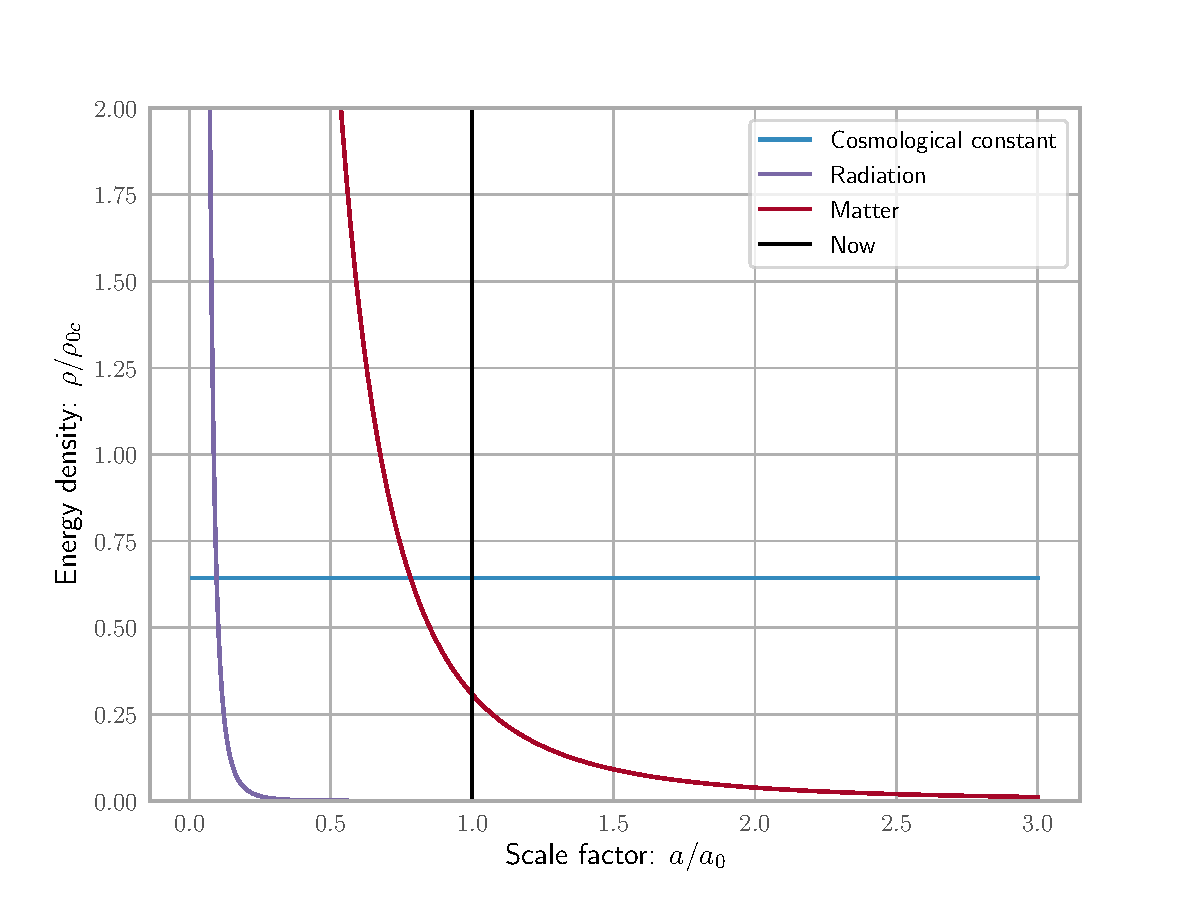
\includegraphics[width=\textwidth]{figures/global_energy_contributions.pdf}
\caption{Contributions to the energy density varying with the scale factor. They are normalized to the current critical energy density, using data from the 2015 Planck mission \cite{PlanckCollaboration:2016XIII}. The increase of the radiation energy density with an increasing scale factor is sharp, but the crossover point with the matter density is at \(a = \rho_{\text{rad}}/\rho_{\text{m}} \approx \num{e-4}\), at which point we have \(\rho \approx \num{e12} \rho_{0c}\).}
\label{fig:global_energy_contributions}
\end{figure}

In this plot, \(a\) can be interpreted as the time, since their relation is monotonic.
We could insert the spatial curvature \(k\) in the plot: it decreases, but slower than matter, since it appears in the first Friedmann equation with an exponent \(a^{-2}\).
We can find an effective \(\rho (a)\) law for the curvature by defining an effective \(\rho_{k}\) for curvature with \(H^2 = \frac{8 \pi G}{3} (\rho + \rho_{k})\), which implies \(\rho_{k} = - 3 k c^2 / (8 \pi G a^2)\). 

We can also express this in units of the critical energy density \(\rho_{c} = 3 H^2 / (8 \pi G)\): we find 
%
\begin{align} \label{eq:spatial-curvature-effective-density}
\frac{\rho_{k}}{\rho_{c}} = - \frac{kc^2}{H^2a^2}
\,.
\end{align}

Now, the dark energy in the universe is the most important component. It it dominant over matter, radiation, and also dominant over spatial curvature.

\section{Solutions of the Friedmann Equations}
\label{sec:solutions-to-friedmann-equations}

We want to solve the equation system 
%
\begin{align}
\frac{\dot{a}^2}{a^2} &= \frac{8 \pi G}{3} \rho - \frac{kc^2}{a}  \label{eq:friedmann-1-later} \\
\rho (t) &= \rho_{* } \qty(\frac{a(t)}{a_{*}})^{-3 (1+w)}
\label{eq:friedmann-3-later}
\,,
\end{align}
%
which encompasses all of the physical content of the FE, since the second equation can be derived from these two. 

Inserting \eqref{eq:friedmann-3-later} into \eqref{eq:friedmann-1-later} we find:
%
\begin{equation}
  \qty(\frac{\dot{a} }{a})^2 = 
  \frac{8 \pi G}{3} \rho_* \qty(\frac{a}{a_*}) ^{-3 (1+w)} - \frac{kc^2}{a^2}\,.
\end{equation}

\subsection{Einstein-De Sitter models}

As we discussed before, if we had zero spatial curvature (\(k=0\)) then we would find \(\rho = \rho_{c} = 3 H^2 / (8 \pi G )\): so, we define the parameter \(\Omega = \frac{8 \pi G \rho}{3 H^2} = \rho / \rho_C\) which quantifies how close this is to being true: experimentally this is compatible with 1.

The Einstein-de Sitter model is one where we take \(\Omega \equiv 1\): negligible spatial curvature, which is equivalent to setting \(k=0\). So, the equation becomes:
\begin{equation}
  \dot{a}^2 = \underbrace{\frac{8 \pi G}{3} \rho_* a_{*}^{3 (1+w)}}_{A^2} a^{-(1+3w)} 
  \,,
  \marginnote{Set \(k=0\), multiplied by \(a^2\), defined \(A\).}
\end{equation}
%
therefore \(\dot{a} = \pm A a^{-\frac{1+3w}{2}}\), or \(a ^{\frac{1+3w}{2}}\dd{a} = \pm A \dd{t}\). 
We choose the positive sign, since we observe the universe to be expanding. 
This can be integrated directly: the equation is 
%
\begin{align}
\int_{a_{*}}^{a} \widetilde{a}^{\frac{1+3w}{2}} \dd{\widetilde{a}} = A \int_{t_{*}}^{t} \dd{\widetilde{t}} = A\qty(t-t_{*})
\,,
\end{align}
%
but we must distinguish two cases: either \((1+3w) / 2 =-1\), which is equivalent to \(w = -1\), or not. 
Let us first assume that \(w \neq -1\). Then, we get:

A solution is:
\begin{align}
  \frac{2}{3 + 3w}\eval{a^{\frac{3+3w}{2}}}_{a_{*}}^{a} &= A \qty(t - t_{*})
   \\
   a^{\frac{3 + 3w}{2}}  - a_{*}^{\frac{3+3w}{2}}
   &= \frac{3 (1+w)}{2} \underbrace{\sqrt{\frac{8\pi G}{3} \rho_{*}}}_{H_{*}} a_{*}^{\frac{3 + 3w}{2}} (t - t_{*}) 
   \marginnote{Since \(k=0\) we have \(H_{*}^2 = \frac{8 \pi G}{3} \rho_{*}\)}
   \\  
  a^{\frac{3 +3w}{2}} &= a_{*}^{\frac{3 + 3w}{2}} \qty(1 + \frac{3}{2} (1+w) H_{*} \qty(t - t_{*}))
   \\
  a(t)&= a_{*} \qty(
    1 + \frac{3}{2} (1+w) H_{*} (t - t_{*})
  )^{\frac{2}{3(1+w)}}
\,,
\end{align}
%
which we can couple to the equation for the evolution of the density, by plugging this expression for the scale factor directly into \eqref{eq:friedmann-3-later}:
%
\begin{equation}
\rho(t) = \rho_{*} \qty(1 + \frac{3}{2}(1+w) H_* (t-t_*))^{-2}
\,,
\end{equation}
%
and also the Hubble parameter \(H \propto \sqrt{\rho }\):  
%
\begin{align}
H(t) = H_{*} \qty(1 + \frac{3}{2}(1+w) H_{*}(t-t_{*}))^{-1}
\,.
\end{align}

There is a time where the bracket in \(a(t)\) is zero, which means \(a = 0 \): this corresponds to the Big Bang, so we call it \(t_{\text{BB}}\), defined by
\begin{equation}
1 + \frac{3}{2} (1+w) H_{*} (t_{\text{BB}} - t_* ) = 0
\,.
\end{equation}

Since the curvature scalar is \(R \propto H^2 \propto \rho \),\footnote{This can be shown by a simple argument: we take the trace of the EFE, to get 
%
\begin{align}
g^{\mu \nu } \qty(R_{\mu \nu } - \frac{1}{2} R g_{\mu \nu })
= 8 \pi G g^{\mu \nu } T_{\mu \nu }
\implies -R = 8 \pi G T
\,,
\end{align}
%
where \(R= g^{\mu \nu } R_{\mu \nu }\) and \(T=g^{ \mu \nu } T_{\mu \nu }\) are the traces of the Ricci tensor and of the stress-energy tensor. 
We've shown that \(R \propto T\): so, since \(T \propto \rho \), we have \(R \propto \rho \), but if we also assume that there is no spatial curvature then \(H^2 \propto \rho \), therefore \(R \propto H^2\).}
at \(t_{\text{BB}}\)  the curvature is diverges.

This time can be expressed by inverting the equation: 
%
\begin{align}
t _{\text{BB}} = t_{*} - \frac{2}{3 (1+w)H_{*}}
\,.
\end{align}

Hakwing \& Ellis proved that if \(w>-1/3\) we unavoidably must have a Big Bang.

We can define a new time variable by 
%
\begin{align}
t_{\text{new}} \equiv t-t _{\text{BB}} =  (t - t_{*}) 
% + 2 H_*^{-1} / (3 (1+w))
+ \frac{2}{3 H_{*} (1+w)}
\,.
\end{align}

Using this new variable the \(t_{*}\) simplifies, and we can just write:
\begin{equation}
a \propto t_{\text{new}}\,^{\frac{2}{3(1+w)}}
\,.
\end{equation}

Inserting this new time variable (which we will just call \(t\)), we get that the Hubble parameter is:
\begin{align} 
H(t) &= \frac{1}{a} \dv{a}{t} = \frac{2}{3(1+w)} t^{\frac{2}{3(1+w)}-1} t^{- \frac{2}{3(1+w)}} \\
H(t) &=  \frac{2}{3(1+w) t} \label{eq:einstein-de-sitter-age}
\,,
\end{align}
so we can compute the density:
\begin{align}
\rho(t) &= \frac{3H^2}{8 \pi G} = \frac{3}{8 \pi G} \frac{4}{9 (1+w)^2 t^2} \\
&= \frac{1}{6 (1+w)^2 \pi G t^2}
\,.
\end{align}
% \todo[inline]{Show this explicitly.}
% Some cases are:
% \begin{equation}
%   \begin{cases}
%       w = 0 \implies a \propto t^{2/3}  \\
%       w=1/3 \implies a \propto t^{1/2} \\  
%       w=1 \implies a \propto t^{1/3}  
%   \end{cases}
% \end{equation}

Let us now revisit the cases from before: 
\begin{enumerate}
  \item \(w=0\) is nonrelativistic matter: it has \(a \propto t^{2/3}\), \(\rho = 1 / (6 \pi G t^2)\) and \(H = 2/ (3t)\). 
  
  This yields a prediction for the age of the universe of \(t \approx \SI{9.6}{Gyr}\) (using the Planck data \cite{PlanckCollaboration:2016XIII}): this is not correct, since the actual value is more like \(t \approx \SI{13.8}{Gyr}\), but it has the right order of magnitude; the discrepancy is due to the fact that the assumption of the universe being dominated by nonrelativistic matter is wrong. 
  \item \(w=1/3\) is radiation: it has \(a \propto t^{1/2}\), \(\rho \propto 3/ (32 \pi G t^2)\) and \(H = 1/ (2t)\);
  \item \(w=-1\) is dark energy: as we mentioned before, this is the case which must be treated separately. The integral yields: 
  %
  \begin{align}
  \log \qty(\frac{a}{a_{*}}) = A (t-t_{*})
  \,,
  \end{align}
  %
  which means 
  %
  \begin{align}
  a (t) = a_{*} \exp(H_{*} a_{*}^{\frac{3 (1+w)}{2}} (t - t_{*}))
  \,,
  \end{align}
  %   
  while, as we saw, \(\rho \) and \(P\) (and, therefore, \(H\)) are constant. 
\end{enumerate}

% The \emph{De Sitter} universe is one where \(w \rightarrow 1\): \(a(t) \propto \exp(Ht) \) and \(H = \const\). (CHECK) 

From the redshift we can trace back the time of emission of the photon: for a matter-dominated universe, for example, we have:
%
\begin{align}
1 + z  = \frac{a_0 }{a} =  \qty(\frac{t_0 }{t})^{2/3}
= \qty(\frac{2}{3H_0 t })^{2/3} 
\,.
\end{align}

We can calculate the deceleration parameter for this case, to check that it is indeed positive: we need to differentiate the expression 
%
\begin{align}
a(t) = a_0 \qty(\frac{3 H_0 t}{2})^{2/3}
\,,
\end{align}
%
and we find 
%
\begin{align}
q_0 = - \frac{\ddot{a}_{0} a_0 }{\dot{a}_{0}^2}
=- \frac{t_0^{-4/3} t_0^{2/3}}{(t_0^{-1/3})^2} \times \frac{\frac{2}{3} \qty(-\frac{1}{3})}{\frac{2}{3} \frac{2}{3}} = \frac{1}{2}
\marginnote{The \(a_0 (3H_0 /2)^{2/3}\) terms all simplify.}
\,.
\end{align}

This is a special case of the fact that \cite[eq. 2.2.4b]{LucchinColes:2002}
%
\begin{align}
q \equiv q_0 = \frac{1 + 3w}{2}
\,.
\end{align}

\end{document}